\begin{figure}[t]
\begin{center}
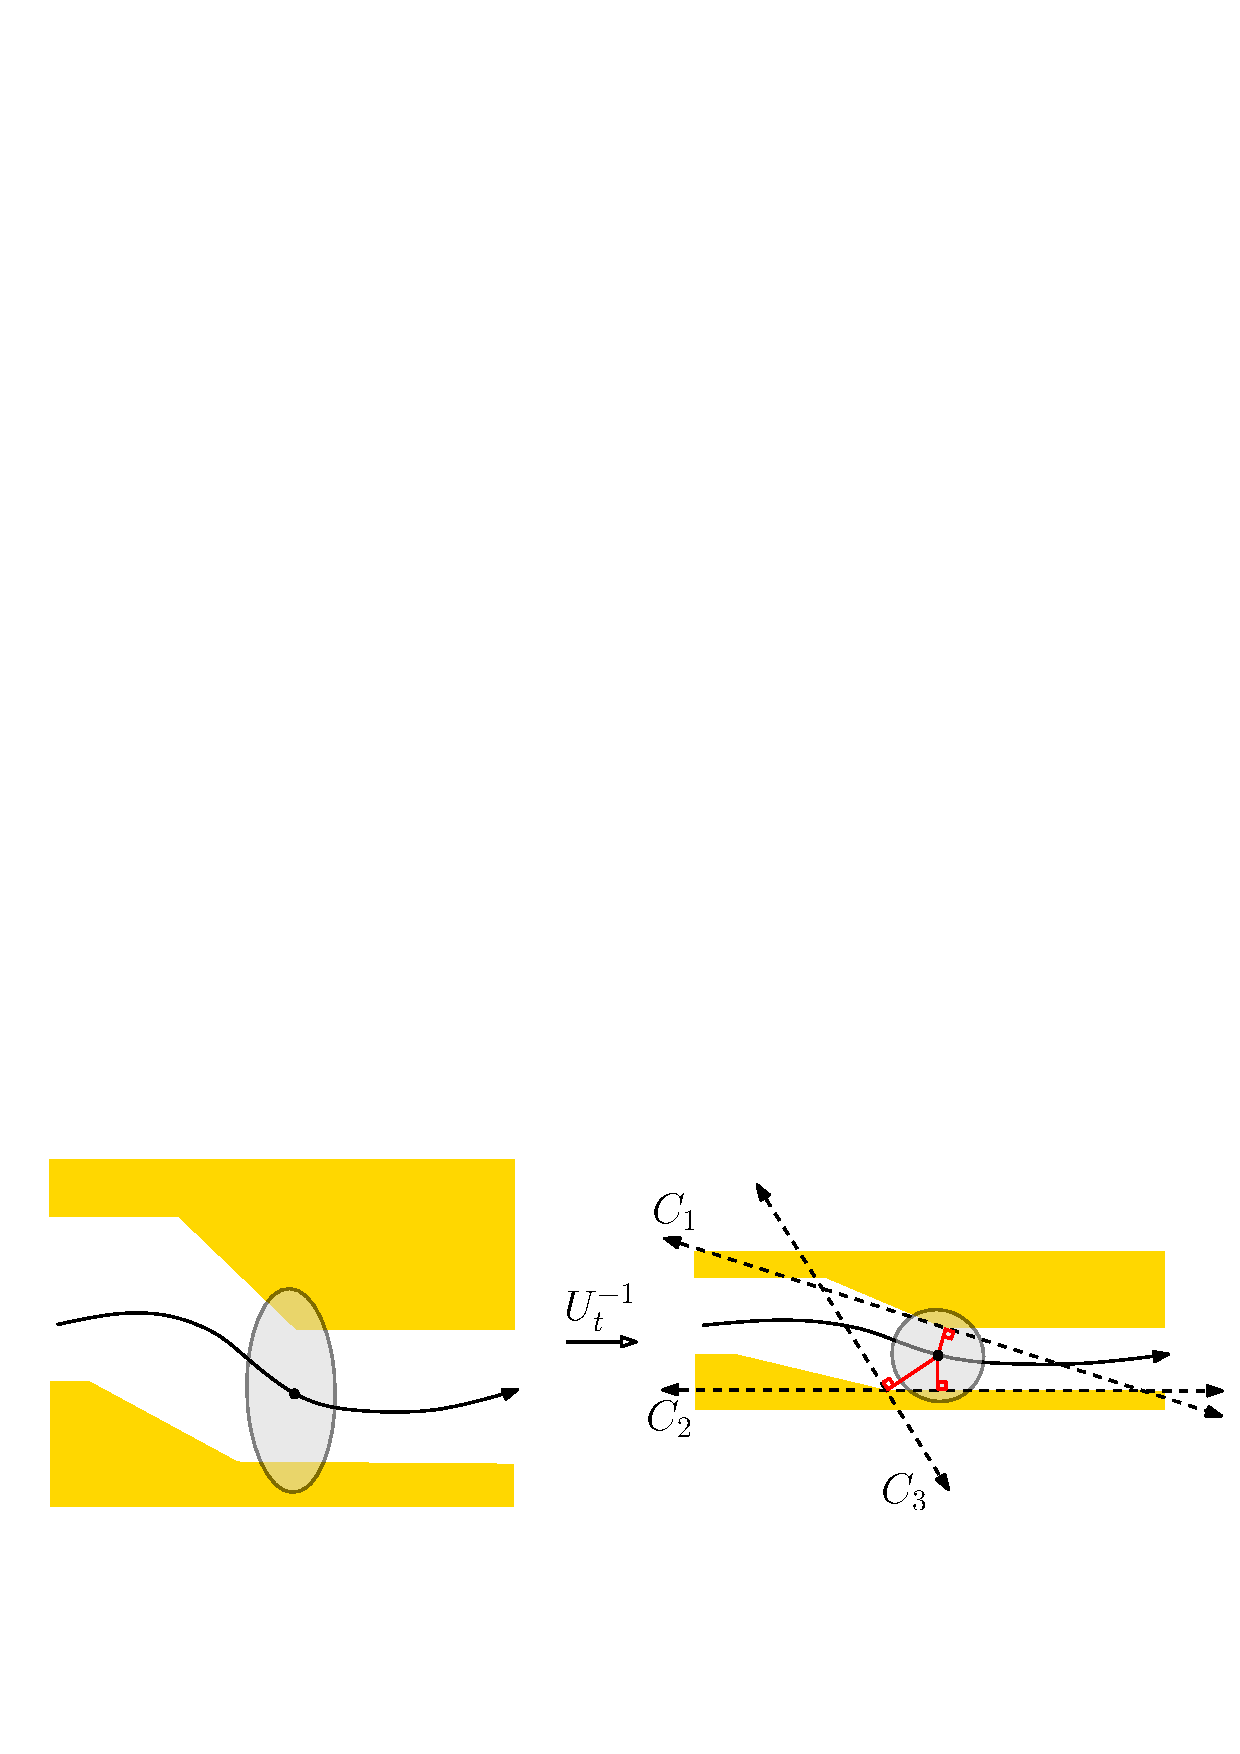
\includegraphics[width=240pt,clip]{figures/convexification.pdf}
\end{center}
\vspace*{-10pt}
\caption{We transform the environment such that the distribution of the robot position (left) is converted to a unit sphere (right). We then sequentially process the obstacle geometry in increasing order of distance from the origin. The linear constraints that define a locally convex region of the free space are determined by the normal to the vector of closest approach (shown in red). The locally convex region constructed using our approach for this example is defined by three constraints determined in order of their indices: $C_1$, $C_2$, and $C_3$.
\vspace*{-10pt}}
\label{fig:convexification}
\end{figure} 

We extend our analysis to non-convex regions by truncating the joint conditional distributions with respect to linear constraints that define a locally convex region of free space containing the robot. For the sake of simplicity, we assume that only the robot position is relevant for collision detection. Given the conditional distribution at stage $t$, $\mathcal{N}[\hat{\mathbf{y}}_{t|t-1} + \bigl[ \begin{smallmatrix} \mathbf{x}^{\star}_t \\ \mathbf{x}^{\star}_t \end{smallmatrix} \bigr], R_{t|t-1}]$, the distribution of the robot position is given by the marginal $\mathcal{N}[\hat{\mathbf{p}}_{t|t-1}, \Sigma_{t|t-1}]$, computed over the state dimensions that describe the robot position. We outline a greedy method that computes a locally convex region of free space such that the probability that the distribution $\mathcal{N}[\hat{\mathbf{p}}_{t|t-1}, \Sigma_{t|t-1}]$ lies beyond the convex region is minimal.

Adopting the approach suggested in \cite{vandenBerg11_IJRR}, we linearly transform the environment geometry by applying the transform $U_t^{-1}$, where $\Sigma_t = U_tU_t^T$ is the Cholesky decomposition. This transforms the uncertainty distribution of the robot position to a Gaussian distribution with zero mean and unit variance, which is a unit sphere in Euclidean space centered at the origin. The spherical symmetry simplifies the task of constructing a nonconservative convex region of free space around the distribution of the position of the robot.

We construct the convex region using a sequential process. We consider the closest point on the obstacle geometry from the origin. The linear truncation constraint $\mathbf{a}_i^T\mathbf{p}_{t|t-1} \leq b_i$, is defined by the normal to the vector of closest approach to the obstacle. We then prune away all geometry that lies in the infeasible half space $\mathbf{a}_i^T \mathbf{p}_{t|t-1} > b_i$ of the constraint, and continue the process by considering the closest point on the remaining obstacle geometry to the origin. This procedure is repeated until all geometry has been pruned away. It is important to note that our convexification method works in a greedy fashion and is not guaranteed to find the least conservative convex bounding region.

In our implementation, we assume that the obstacles are defined in a piecewise linear fashion using either line segments in $\mathbb{R}^2$, or polygons in $\mathbb{R}^3$. We only consider obstacles that are contained within $3$ standard deviations of the distribution (corresponding to a distance of $3$ units from the origin in the transformed environment). Instead of performing a linear-time search by iterating over all obstacles, we use a BSP tree \cite{Book:Berg08} data structure to determine obstacles within the given search radius, in logarithmic time. 